\section{Some example use cases}

\frame{%
    \begin{algorithm}[H]\DontPrintSemicolon%
        \KwIn{%
            A dataset, \(X \in \mathbb{R}^n \times \mathbb{R}^n\);
            \(
                f: \mathbb{R}^n \times \mathbb{R}^n \to \mathbb{R},\quad
                f(A, B) = Var(A) - \max_i \left|B_i - 1\right|
            \)
        }
        \KwOut{The \alert{maximal} value for \(f\)}\;

        \(values \gets \emptyset\)\;
        \For{each ordering, \(a, b \in {\{0, 1\}}^2\), of the columns}{%
            calculate \(f\left(X^{(a)}, X^{(b)}\right)\)\;
            append this to \(values\)\;
        }

        \KwRet{\(\max values\)}
    \end{algorithm}
}

\frame{%
    \centering
    \begin{figure}
        \animategraphics[%
            loop,controls,width=\textwidth%
        ]{1}{img/circle/epoch_}{0}{100}
    \end{figure}
}

\frame{%
    \centering
    \begin{figure}
        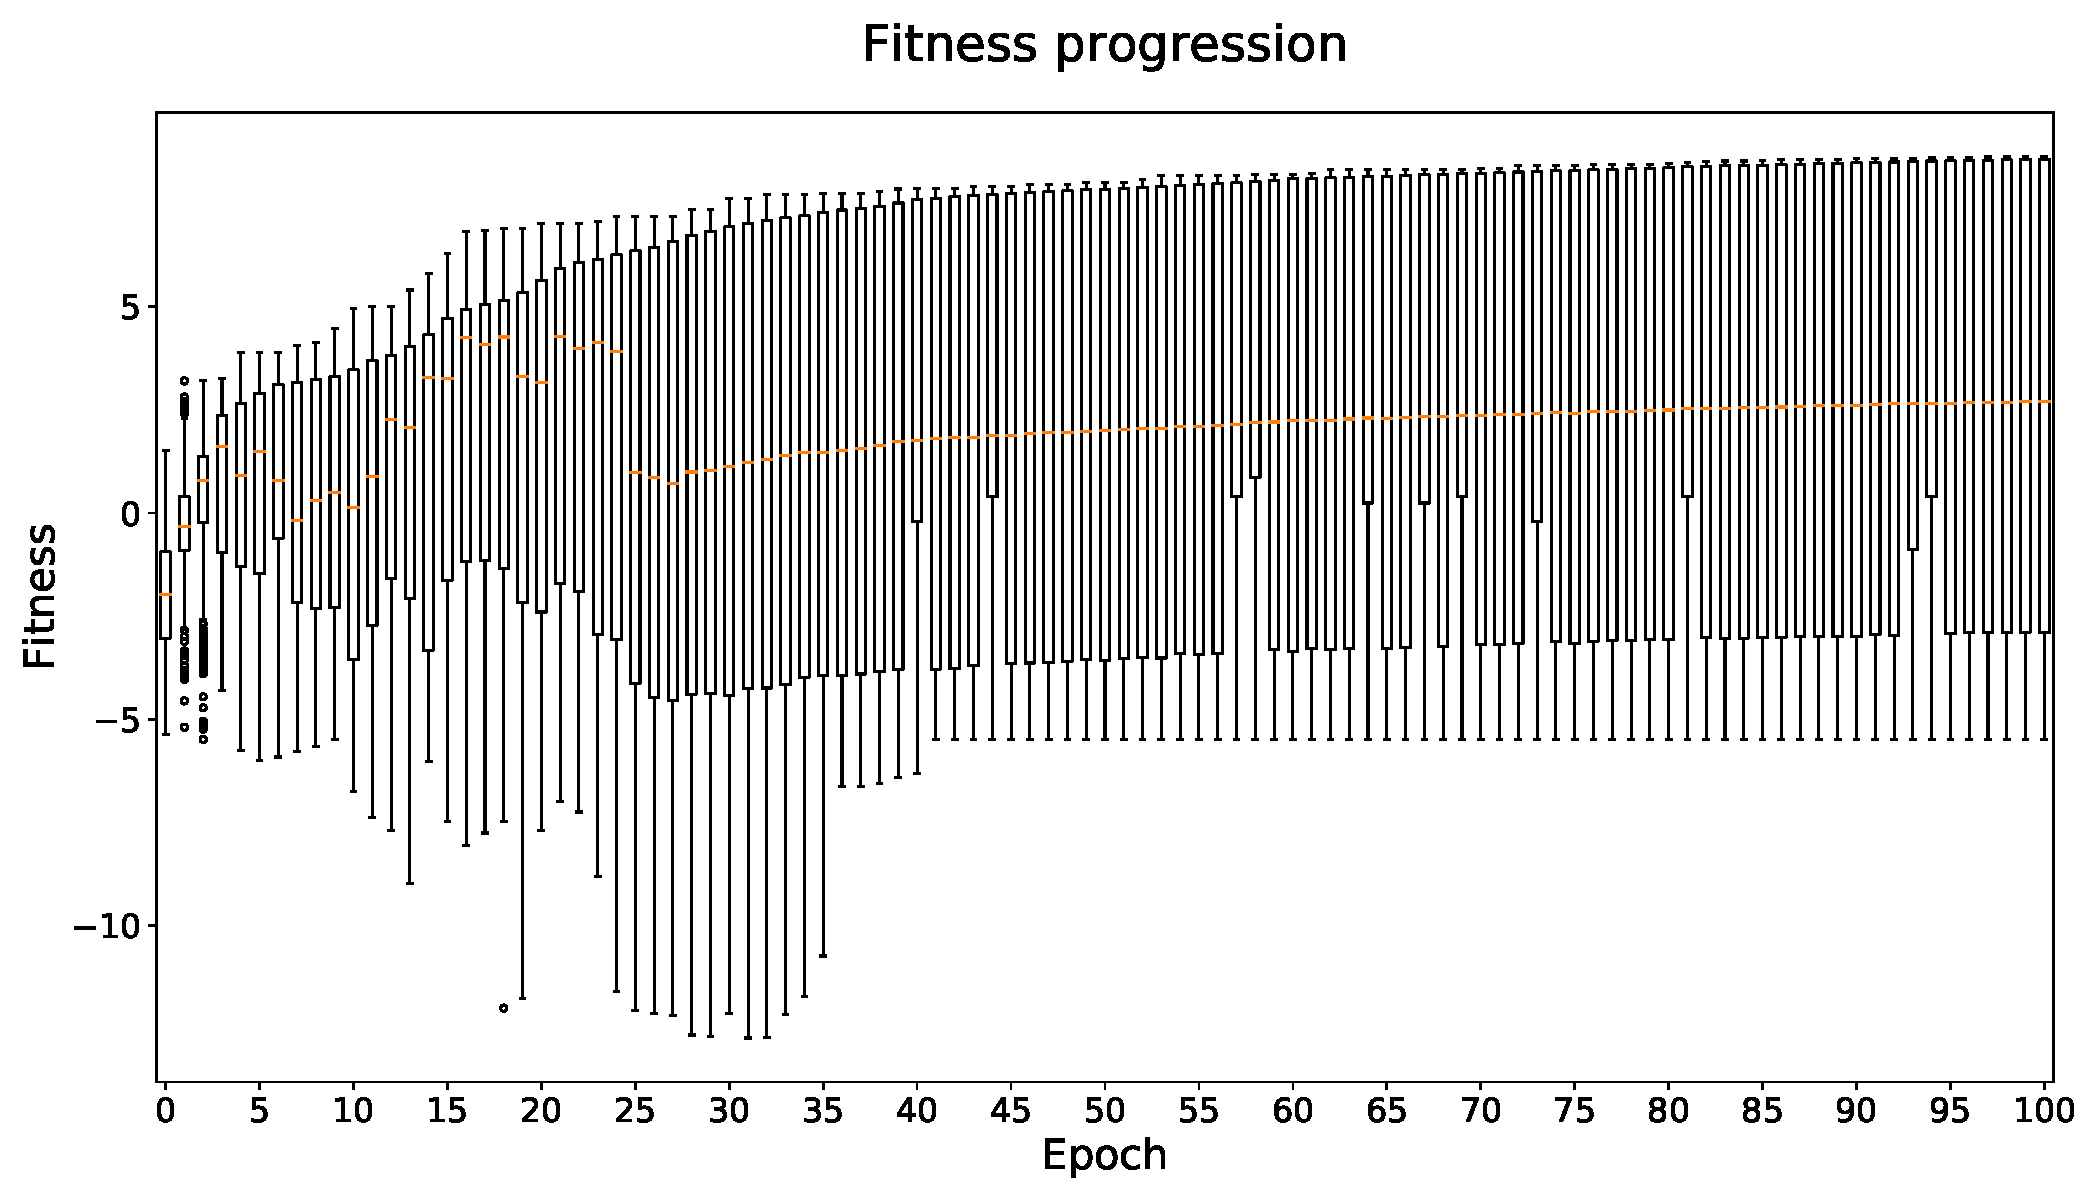
\includegraphics[width=\textwidth]{img/circle/fitness.pdf}
    \end{figure}
}

\frame{%
    \begin{algorithm}[H]\DontPrintSemicolon%
        \KwIn{%
            A dataset, \(X \in \mathbb{R}^n\);
            some sampling proportion, \(p \in [0, 1]\);
            a number of samples to take, \(k\)
        }
        \KwOut{%
            The maximum \alert{difference} between each sampled mean of \(X\)
            and 0
        }\;

        \(values \gets \emptyset\)\;
        \For{\(i = 1, \ldots, k\)}{%
            \(Y \gets\) a random sample of \(\left\lfloor np \right\rfloor\)
            entries from \(X\)\;
            evaluate the mean of \(Y\):
            \[
                \bar Y = \frac{1}{|Y|} \sum_{i=1}^{|Y|} Y_i
            \]
            append \(\bar Y\) to \(values\)
        }

        \KwRet{\(\max values\)}
    \end{algorithm}
}

\frame{%
    \centering
    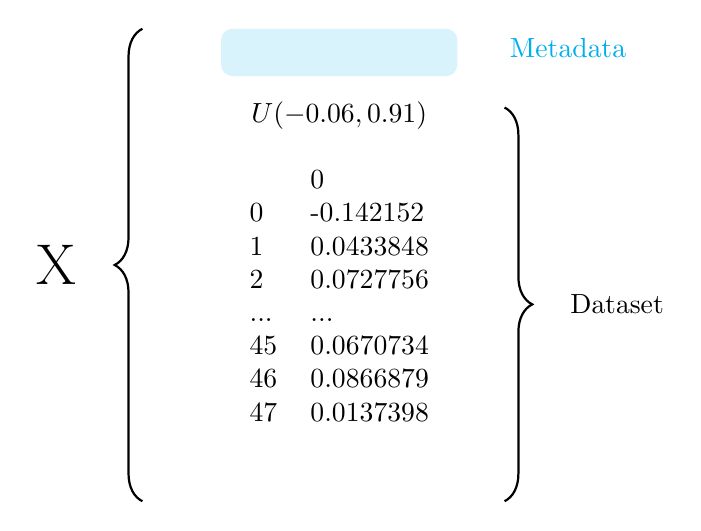
\begin{tikzpicture}

        \fill[cyan!15, rounded corners] (-1.5, 2.4) rectangle (1.5, 3)
            node[right=40pt, below] {\color{cyan} Metadata};
        \node at (0, 0) {%
            \begin{tabular}{c}
                \(U(-0.06, 0.91)\)\\
                {}\\
                \begin{tabular}{ll}
\toprule
{} &          0 \\
\midrule
0   &  -0.142152 \\
1   &  0.0433848 \\
2   &  0.0727756 \\
... &        ... \\
45  &  0.0670734 \\
46  &  0.0866879 \\
47  &  0.0137398 \\
\bottomrule
\end{tabular}

            \end{tabular}
        };

        \draw[decorate, decoration={brace, amplitude=10pt}, thick]%
            (-2.5, -3) -- (-2.5, 3) node[midway, left=20pt] {\huge X};
        \draw[decorate, decoration={brace, amplitude=10pt}, thick]%
            (2.1, 2) -- (2.1, -3) node[midway, right=20pt] {Dataset};
    \end{tikzpicture}
}

\frame{%
    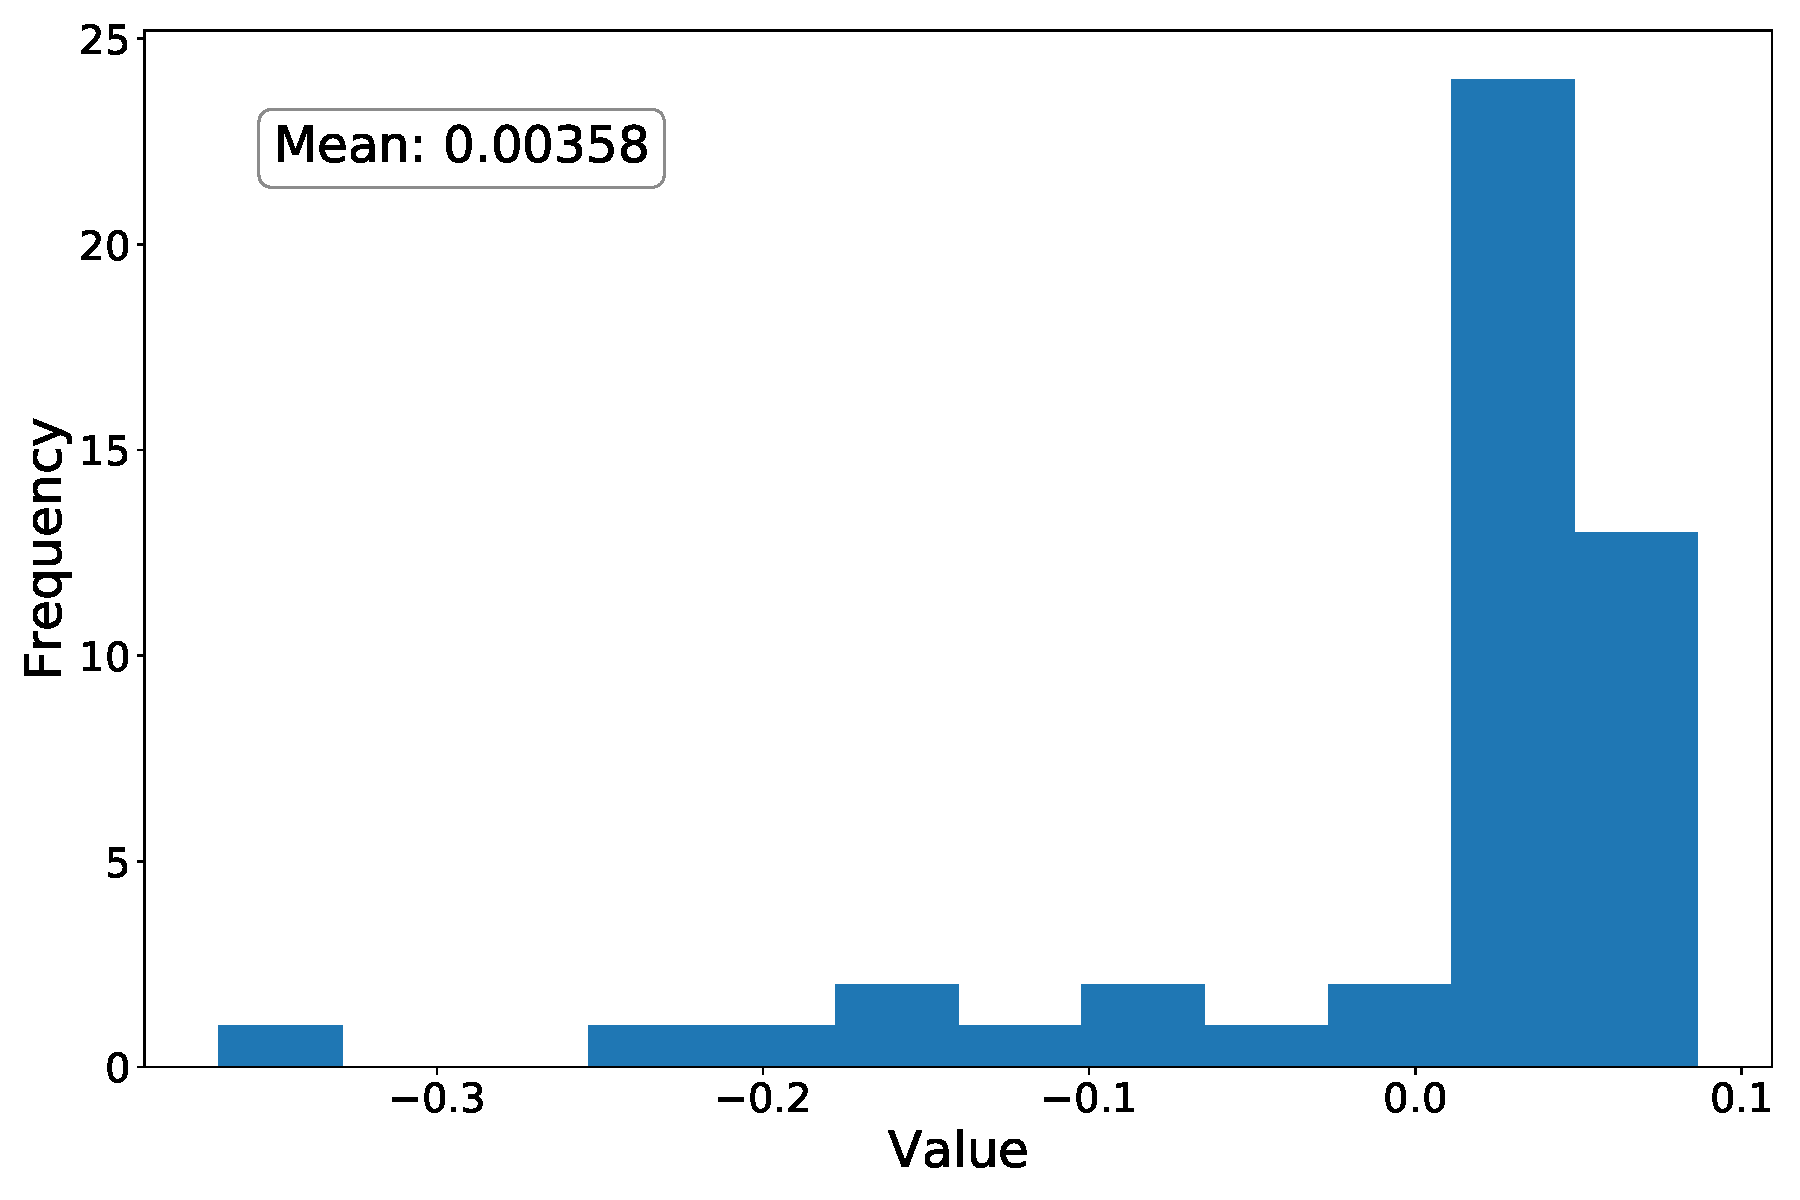
\includegraphics[width=\textwidth]{img/sample_mean.pdf}
}

\frame{%
    \begin{algorithm}[H]\DontPrintSemicolon%
        \KwIn{%
            A dataset, \(X \in \mathbb{R}^n \times \mathbb{R}^n\);
            a set of \alert{dissimilarity} measures, \(%
                f_1, \ldots, f_k:
                \mathbb{R}^n \times \mathbb{R}^n \to \mathbb{R}
            \)
        }
        \KwOut{The total of the measures: \(\sum_{i=1}^k f_i(X)\)}\;

        \(sum \gets 0\)\;
        \For{\(i = 1, \ldots, k\)}{%
            evaluate \(f_i(X)\)\;
            add this to \(sum\)\;
        }

        \KwRet{\(sum\)}
    \end{algorithm}
}

\frame{%
    \centering{%
        \(X\) Mean: 5 \hfill%
        \(Y\) Mean: 7 \hfill%
        \(X\) Std.: 4.7 \hfill%
        \(Y\) Std.: 4.1 \hfill%
        Corr.: 0.8
    }\vfill

    \begin{minipage}{\linewidth}
        \hspace*{-30mm}
        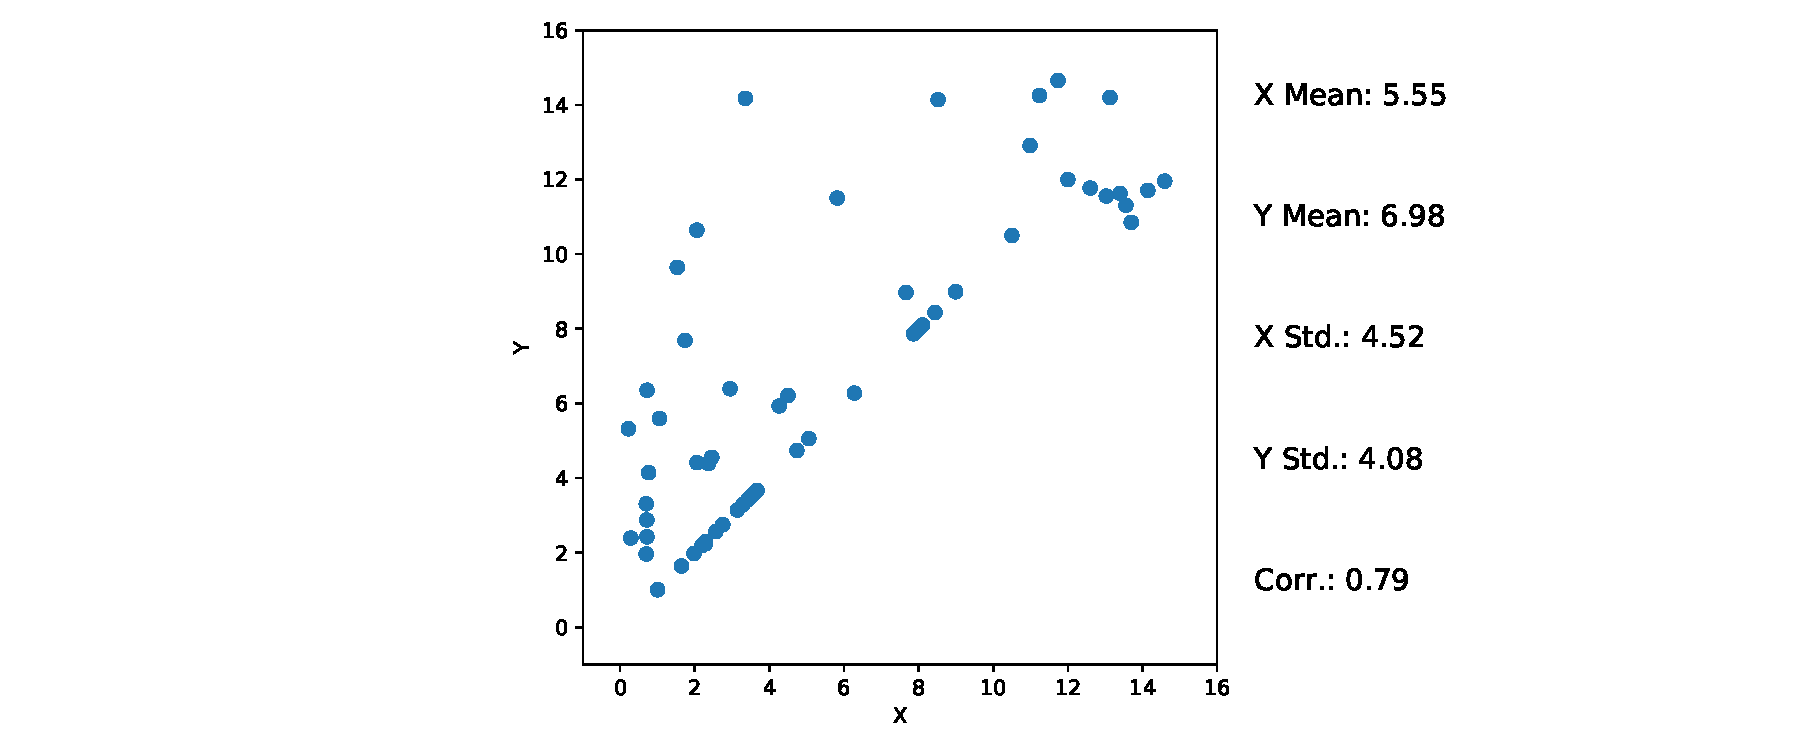
\includegraphics[height=.4\paperheight]{img/anscombe/best_0.pdf}%
        \hspace*{-30mm}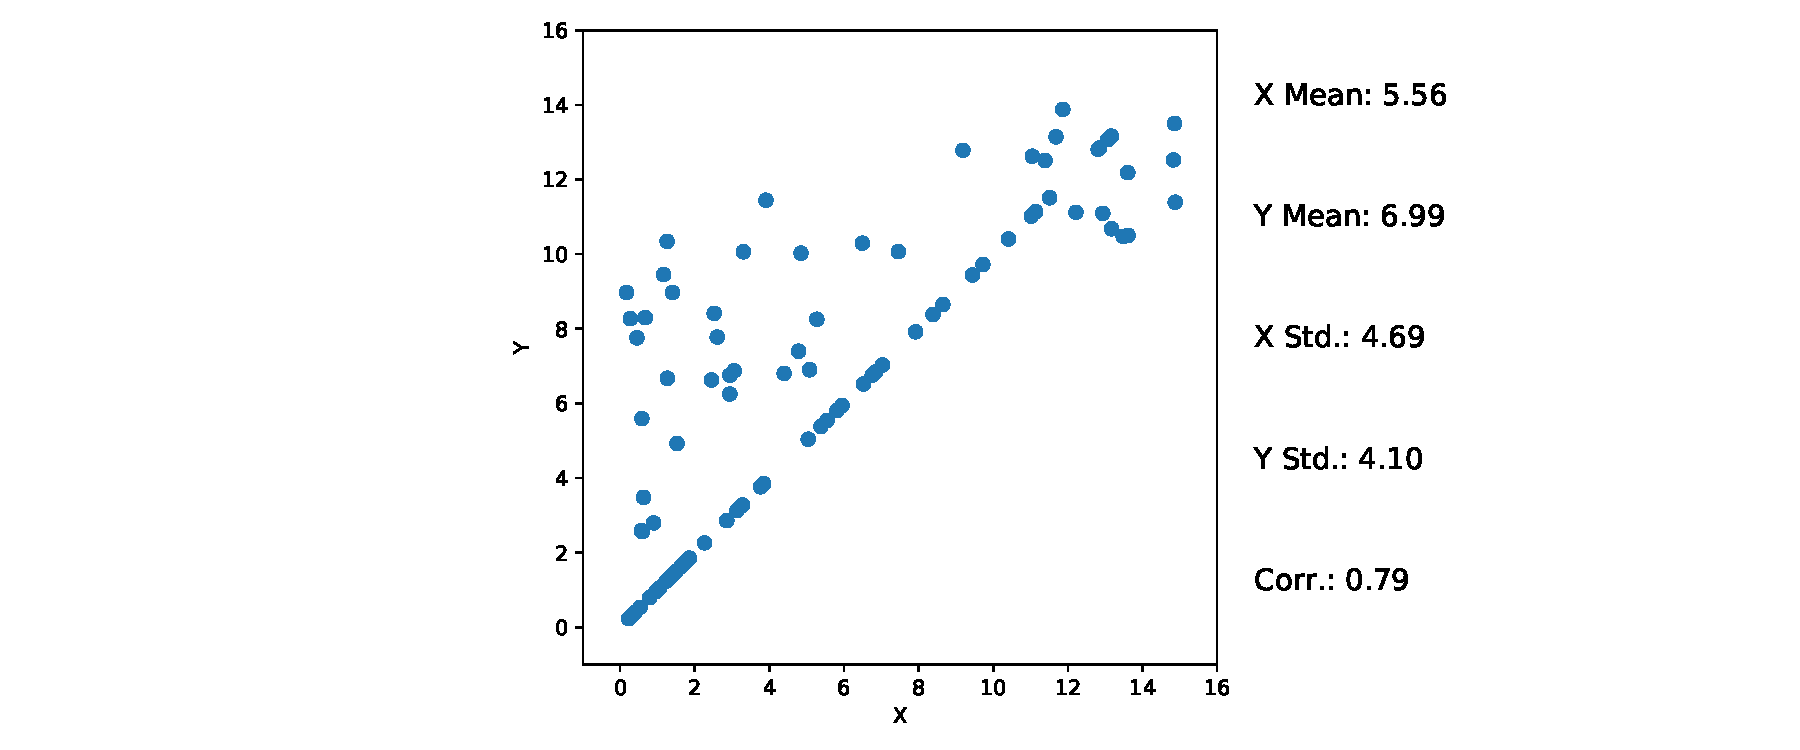
\includegraphics[height=.4\paperheight]{img/anscombe/best_1.pdf}
    \end{minipage}
    \begin{minipage}{\linewidth}
        \hspace*{-30mm}
        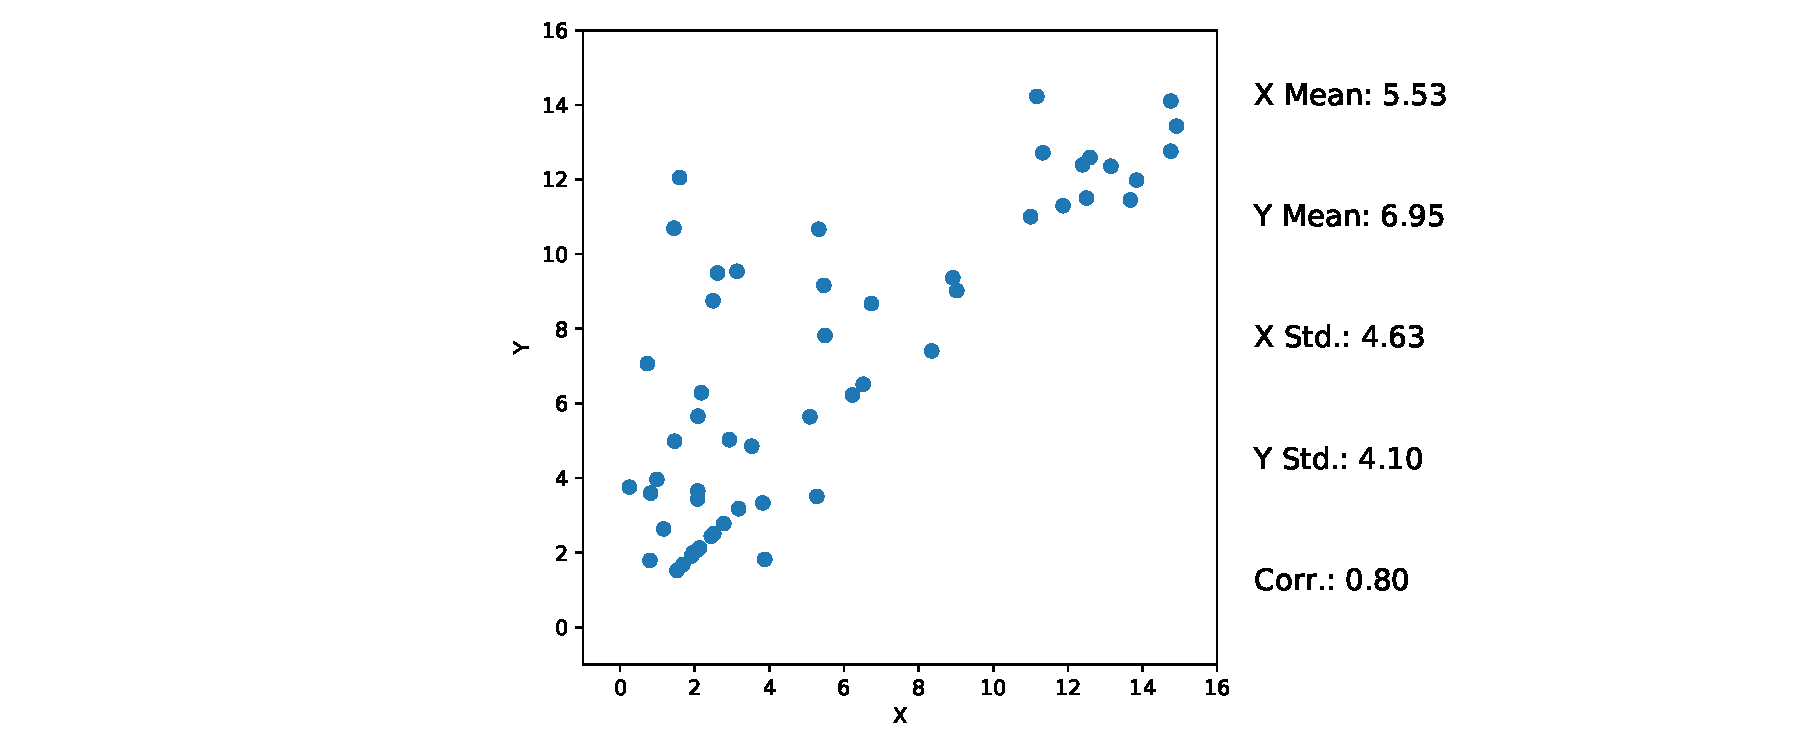
\includegraphics[height=.4\paperheight]{img/anscombe/best_2.pdf}%
        \hspace*{-30mm}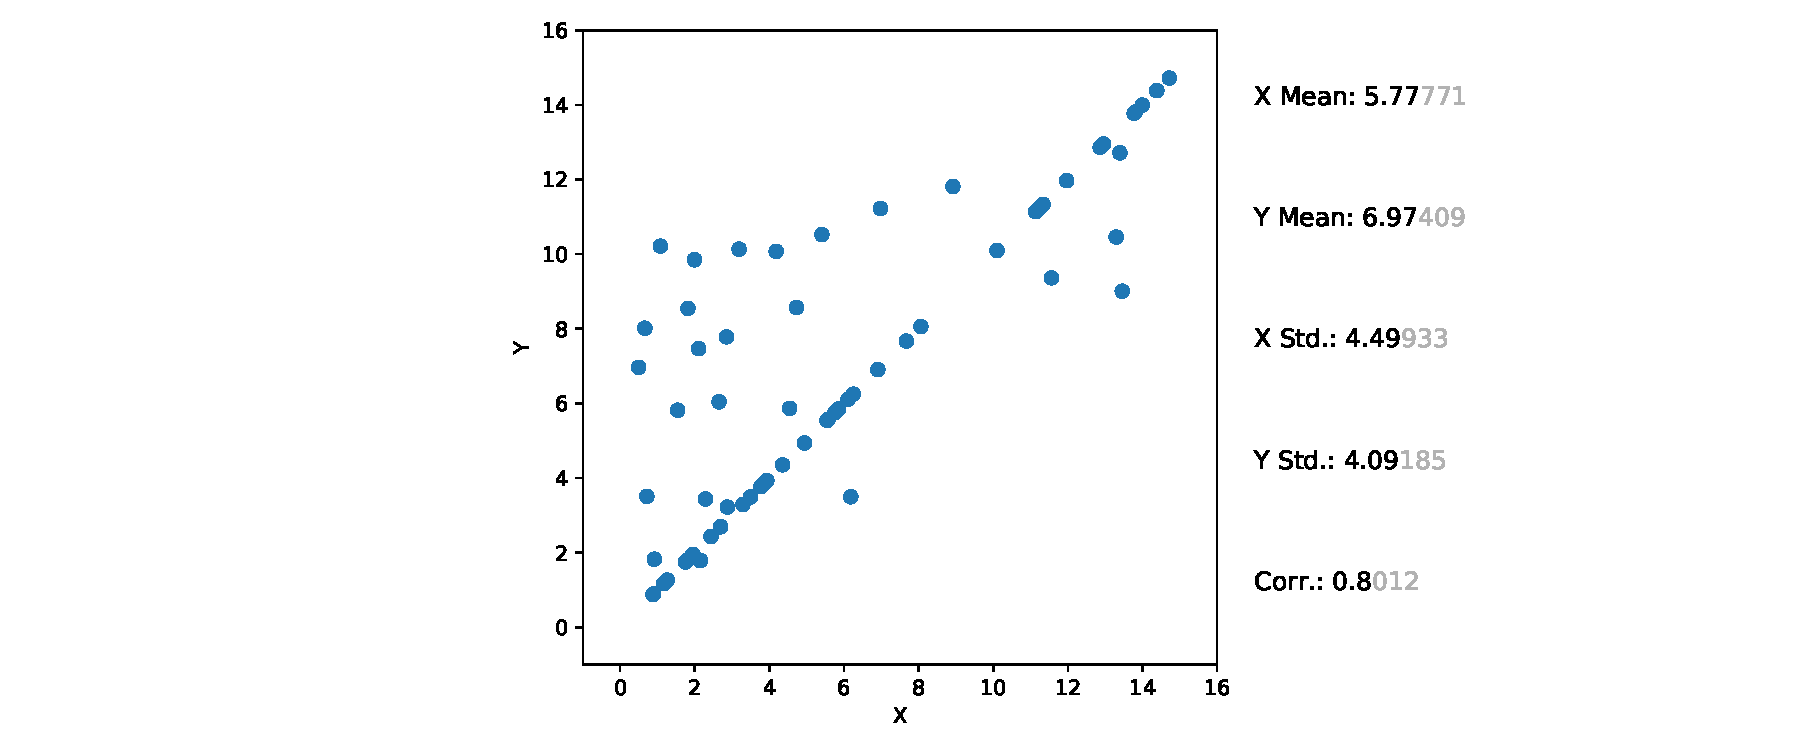
\includegraphics[height=.4\paperheight]{img/anscombe/best_3.pdf}
    \end{minipage}
}

\frame{%
    \begin{figure}
        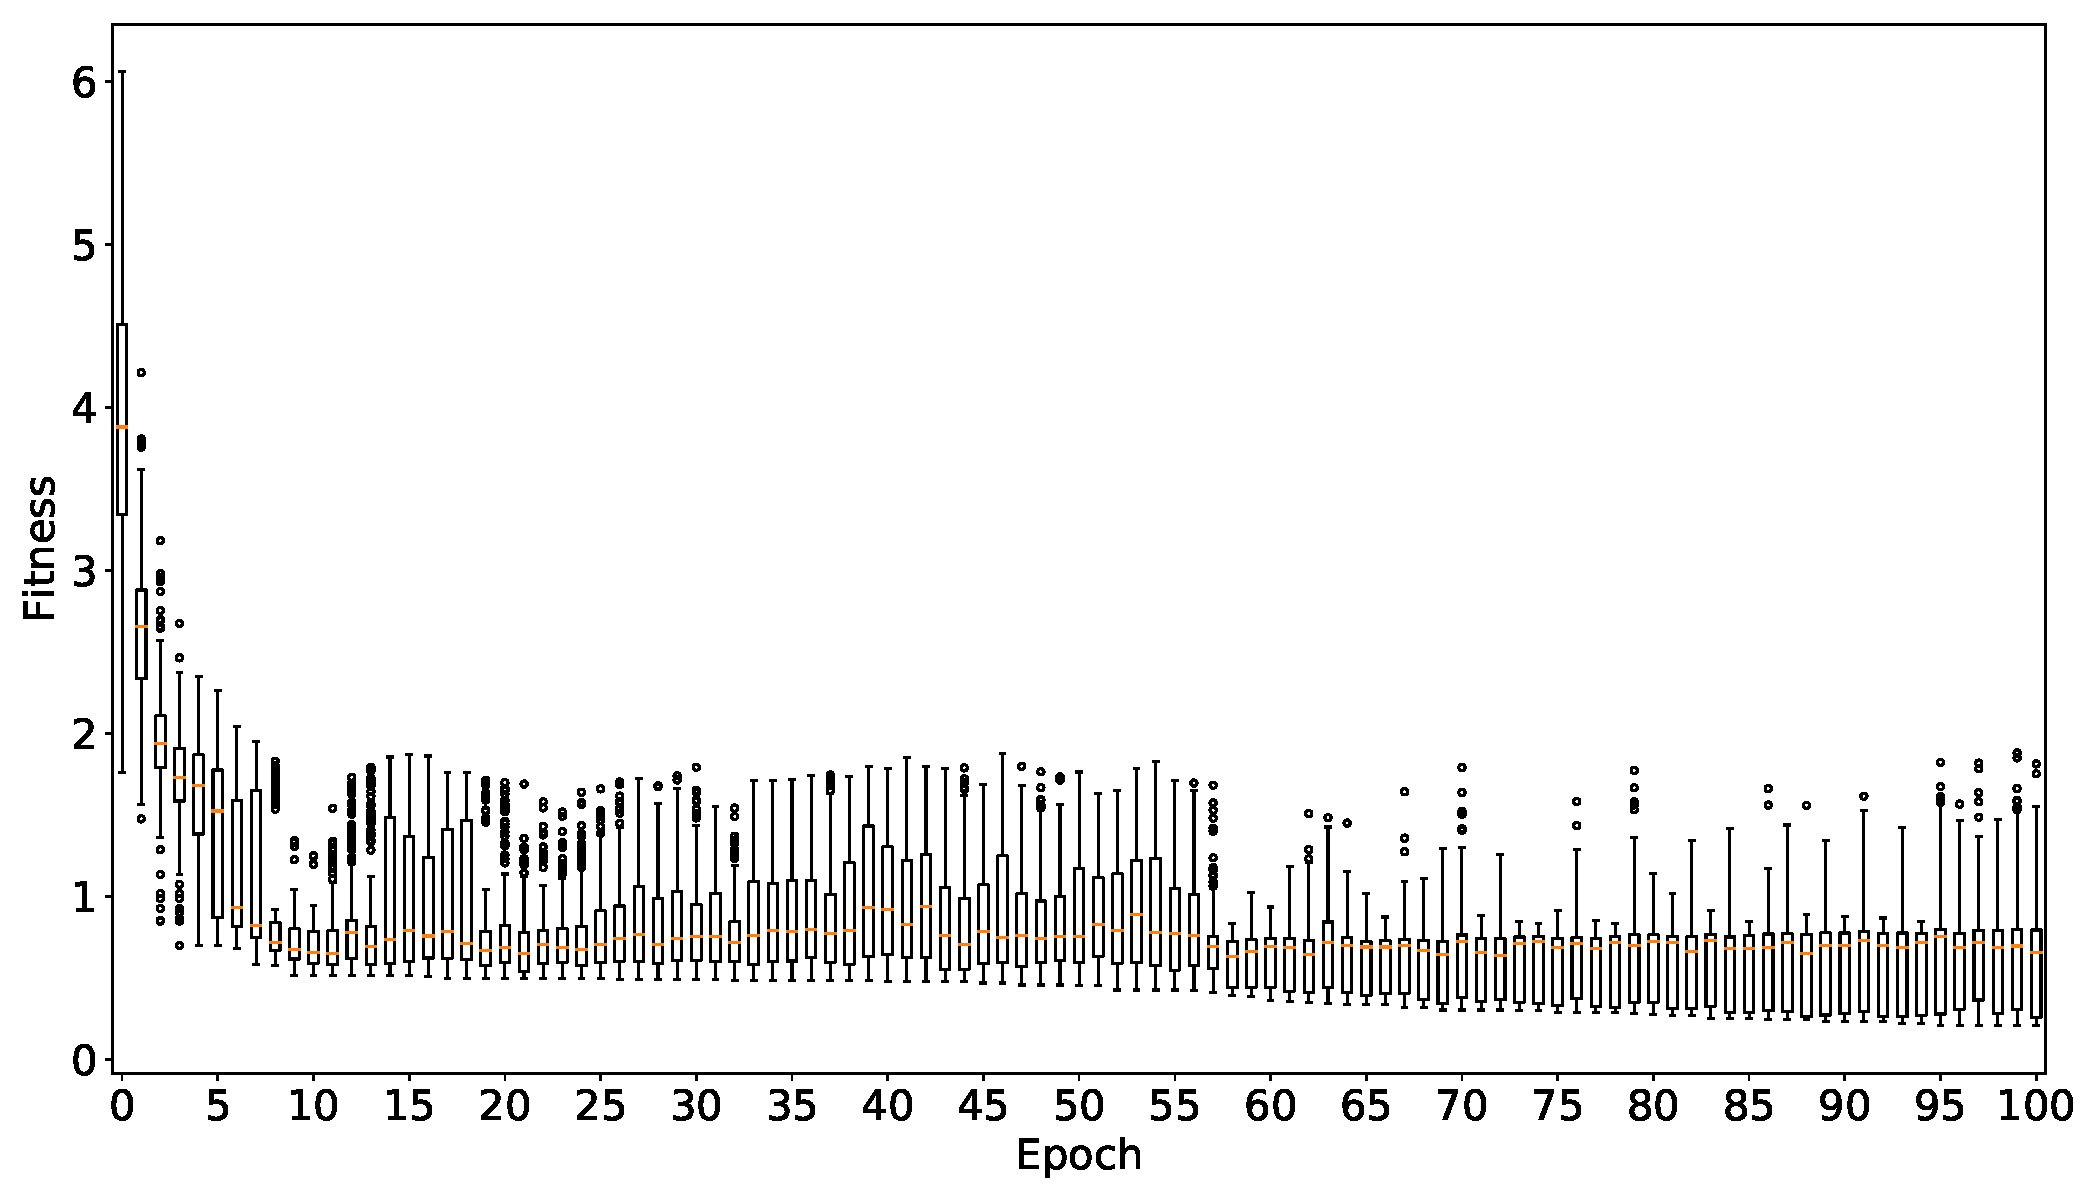
\includegraphics[width=\textwidth]{img/anscombe/fitness.pdf}
    \end{figure}
}

\hammerpage%
